\subsection{Life cycle of a ShowOff module}

Upon launch, Launcher parses the command line. It decides that a ShowOff must
be started. This will read the parameters stored in Psyclone. The available
parameter names are:

\begin{itemize}
 \item[Attractors] A comma-separated list of attractors which are specified as
                   $\langle$name$\rangle$:$\langle$weight$\rangle$.
\end{itemize}

After this, the ShowOff goes into a waiting loop, expecting stories and
analyses on their respective whiteboards. When a story is received, a particle
is created, when an analysis is received, the accompanying story is searched
for and the particle is updated accordingly (attraction parameters are
updated).

\begin{figure}[htp]
  \centering
  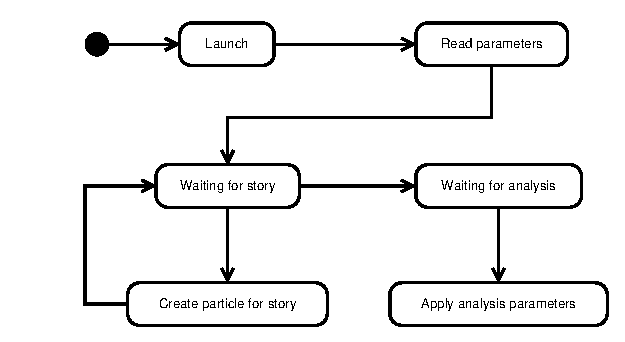
\includegraphics{image/sequence-diagram-showoff}
  \caption{Sequence diagram of a ShowOff module}
\end{figure}
